
\section{Theory}

% \section{Single Particle Dynamics}
% \label{sec:single_particle_dynamics}

% To derive the method used in simulating the beam, it is usefull to start with
% Maxwell's equations. These can be used to describe the motion for charged
% particles under the magnetic fields of accelerator components, such as dipoles
% and quadrupoles. The solutions to these equations become increasingly complex at
% higher perturbations so it is usefull to devise a coordinate system other than

% Specifying a coorindate system such that the origin follows the ideal path of
% the particle beam, rather than a coordinate system about an arbitary fixed
% point we are able to describe the state of a patricle by

% \begin{equation}
% 	\begin{pmatrix}
% 		x(z) \\ x'(z) \\
% 		y(z) \\ y'(z) \\
% 	\end{pmatrix}
% 	=
% 	\begin{pmatrix}
% 		C_x(z)  & S_x(z)  & 0 & 0 \\
% 		C'_x(z) & S'_x(z) & 0 & 0 \\
% 		0 & 0 & C_y(z)  & S_y(z)  \\
% 		0 & 0 & C'_y(z) & S'_y(z) \\
% 	\end{pmatrix}
% 	\begin{pmatrix}
% 		x_0 \\ x'_0 \\
% 		y_0 \\ y'_0 \\
% 	\end{pmatrix}
% \end{equation}

% where \(x\) and \(y\) are deviations form the centre of the beam along their
% respective axis and \(x'\) and \(y'\) are the transverse momenta of the
% particle perpendicular to \(z\), the direction of travel of the beam.
% Transformations in either the $x$ or $y$ plane are independent, however, it is
% clear that coupling effects can still be included
% % TODO

\subsection{Single Particle Dynamics}

When working with beams of particles, it is advantagous to work in the
coordinate system that follows the ideal path of the beam. If the beam's motion
in the \(x\) and \(y\) planes are independent, i.e. we ignore coupling terms,
the each particle's motion in each plane can be described by
\begin{equation}
	\begin{pmatrix}
		u(z) \\ u'(z)
	\end{pmatrix}
	=
	\begin{pmatrix}
		C_u(z)  & S_u(z)  \\
		\sqrt{C'_u(z)} & S'_u(z)
	\end{pmatrix}
	\begin{pmatrix}
		u_0 \\ u'_0
	\end{pmatrix}
\end{equation}
where \(u\) is either \(x\) or \(y\) and \(u'\) is the transverse velocity of
the particle in the \(u\) plane. The coordinate \((u, u')\) lies in what is
known as phase space. Using this system of matricies the drift and quadrupole
matricies can be derived \cite{wiedemann2007particle}. The drift matrix is
\begin{equation}
	\mathcal{M}_D(l) =
	\begin{pmatrix}
		1 & l \\
		0 & 1
	\end{pmatrix} \\
\end{equation}
the focusing quadrupole matrix is
\begin{equation}
	\mathcal{M}_{QF}(l) =
	\begin{pmatrix}
		\cos\psi & \frac{1}{\sqrt{k}}\sin\psi \\
		-\sqrt{k}\sin\psi & \cos\psi
	\end{pmatrix} \\
\end{equation}
and the defocusing quadrupole matrix is
\begin{equation}
	\mathcal{M}_{QD}(l) =
	\begin{pmatrix}
		\cosh\psi & \frac{1}{\sqrt{\abs{k}}}\sinh\psi \\
		-\sqrt{\abs{k}}\sinh\psi & \cosh\psi
	\end{pmatrix}
\end{equation}

These transport matricies can be multiplied together resulting in the
transformation matrix representing a path containing all accelerator components
making it simple to follow a particle through a transport line.

\subsection{Emittance}

\begin{figure}
	\centering
	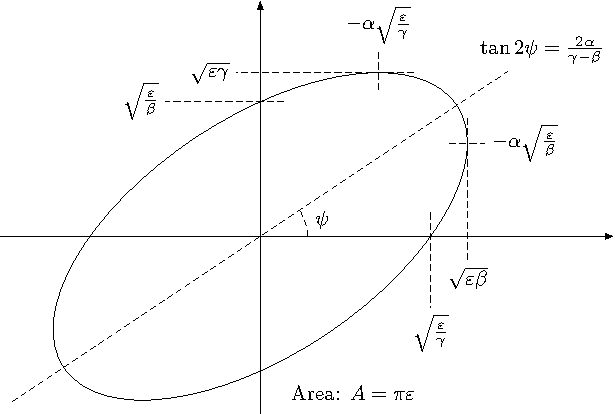
\includegraphics{figures/ellipse}
	\caption{
		A representation of the relation between the Twiss parameters of
		a beam's ellipse in phase space~\cite{wiedemann2007particle}.}
	\label{fig:ellipse}
\end{figure}

Grouping the individual particles in a particle beam, they will occupy an area
in phase space known as the emittance.  Qualitatively the emittance of a beam is
a measure of how parallel the particles of the beam are to each other. It is a
conserved quantity while the beam is not being acted upon by external forces.

In phase space the beam of particles will usually take up an area resembling
that of an ellipse. This is because, after a diverging or converging beam has
traveled through an apeture, we expect particles that are further away from the
centre of the beam to have a larger transverse momentum. This is unless the beam
is being measured at it's waist where it is transitioning between converging and
diverging or visa versa. Figure~\ref{fig:ellipse} shows the projection of a
diverging beam onto a two dimensional phase plane, called the phase ellipse.
The line that defines the ellipse is drawn such that \SI{95}{\percent} of all
the particles in the beam are contained~\cite{buon1994beam}. The emittance is
defined by the area of this ellipse divided by \(\pi\) in units of
\si{\meter\radian}. Note that in general the transverse momenta, hence the slope
of the particles in the beam, are very small so the approximation \(\sin
u'\approx u'\) can be used.

% \begin{equation}
% 	\int_{\text{ellipse}}\mathrm{d}x\mathrm{d}x' =\pi\epsilon
% \end{equation}

The general equation of an ellipse can be used to describe the phase ellipse:
\begin{equation}
	\gamma x^2 + 2\alpha xx' + \beta x'^2 = \epsilon
\end{equation}
where \(\alpha\),  \(\beta\), \(\gamma\) and \(\epsilon\) are ellipse parameters
that determine the ellipse's shape and orientation in phase space, where
\(\epsilon\), the area of the ellipse is the emittance~\footnote{Often, the
units of \(\pi\) are omitted and the emittance is given in units of
\si{\pi\;\meter\;\radian}.} Of the four beam parameters, only three are
independant and since \(\epsilon\) is defined as the area, the other three can
be found to be correlated from the ellipse's geometric properties by
\begin{equation}
	\beta\gamma - \alpha^2 = 1
\end{equation}

% \subsection{Methods of measurement}

% The phase-space density and emittance of a beam must be infered from beam
% profiles captured using charge-coupled device (CCD) cameras after undergoing
% spatial filtering.

By expressing this ellipses as a matrix, transformation rules have been derived
to transport the beam~\cite{wiedemann2007particle}. The beam matrix can be
defined by
\begin{equation}
	\bm{\sigma} =
	\begin{pmatrix}
		\sigma_{11} & \sigma_{12} \\
		\sigma_{21} & \sigma_{22} \\
	\end{pmatrix}
	=
	\epsilon
	\begin{pmatrix}
		\beta & -\alpha \\
		-\alpha & \gamma \\
	\end{pmatrix}
\end{equation}
where each element describes distributions of particles in the beam as follows:
\begin{align}
	\sigma_{11} &= \langle x_i^2 \rangle = \epsilon\beta \\
	\sigma_{22} &= \langle {x'}_i^2 \rangle = \epsilon\gamma \\
	\sigma_{12} &= \langle x_i x'_i \rangle = -\epsilon\alpha
\end{align}

The evolution of this matrix along the beam transport line can then be described
by
\begin{equation}
	\bm{\sigma}_1 = \mathcal{M}\;\bm{\sigma}_0\;\mathcal{M}^T
	\label{eq:apply}
\end{equation}

% TODO measurement of the emittance 183gg (page 164)
